\section{Introduction}
\label{sec:intro}

\begin{figure*}[!tb]
\centering
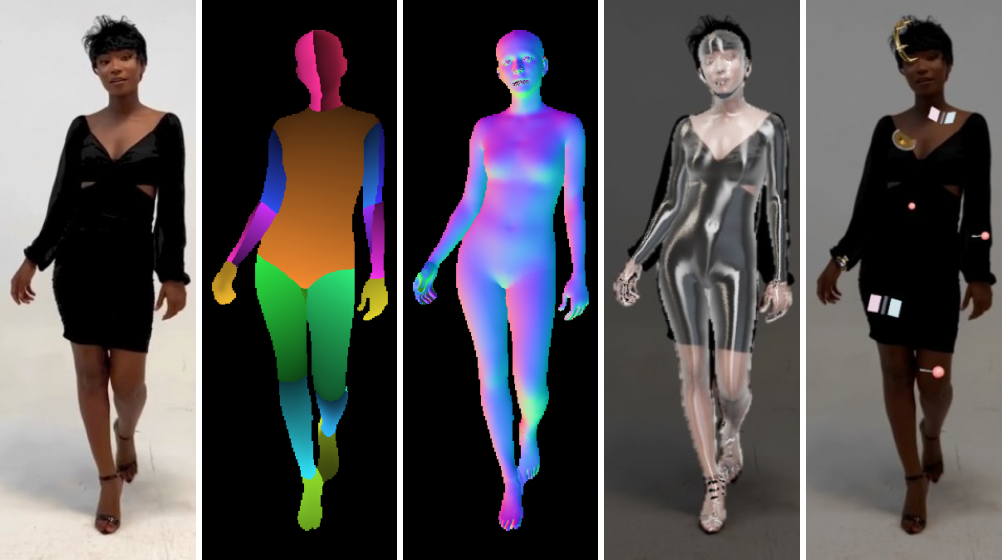
\includegraphics[width=0.42\linewidth]{figs/fig_teaser.png}
\caption{\textbf{Oriented DensePose.} Per pixel, in one pass: the correspondence $(I,U,V)$
\emph{and} a surface frame $\hat R\in SO(3)$; then $\hat R\,\mathbf{n}_{T}$ as a camera-space normal
map, smooth across part seams; satin whose highlight \emph{direction} is set by the twist of
$\hat R$ about the normal; and objects attached at clicked pixels and oriented by $\hat R$.}
\label{fig:teaser}
\end{figure*}

DensePose~\cite{guler2018densepose} defined a task a large family of human-centric systems now
takes for granted: for every foreground pixel of a person, name the point of a canonical body
surface that projects there. Its output --- a part index and two chart coordinates, $(I,U,V)$ ---
became an unusually durable interface, consumed by pose-guided synthesis, garment transfer, avatar
reconstruction and video
re-animation~\cite{neverova2018dpt,pidm2023,cfld2024,fpdm2024,mcld2025,leffa2025}. Those consumers
have been rebuilt more than once, and DensePose accuracy work did
continue~\cite{yang2019parsingrcnn,neverova2019slim,neverova2020cse} --- but the predictor they
import is, overwhelmingly, the detectron2 ResNet-101 released in 2019~\cite{wu2019detectron2}. We
revisit the producer, asking whether its \emph{output} is rich enough, and find that answering that
forces a second question, whether its \emph{supervision} is correct.

\paragraph{The output.}
A correspondence says where a pixel lies, not how the surface is turned there: a template point has
two degrees of freedom, and a frame there adds the three rotational ones. We predict per pixel a
rotation $R\in SO(3)$ carrying the template's own surface frame at the corresponding point into the
camera frame, so $R\,\mathbf{n}_{T}$ is the camera-space normal, $R\,\mathbf{t}$ transports any
template tangent --- the direction a hair or woven fibre runs --- and $R$ in full supplies the
twist about the normal, which a normal map cannot express but which separates a satin highlight or
an object glued to a moving limb from a plausible-looking smear (\cref{fig:teaser}). Anchored to
the template rather than the chart, the frame is \emph{chart-independent}: continuous across seams
and unchanged by a re-cut of the atlas.

\paragraph{The supervision.}
Predicting a frame is what forced us to fix the correspondence, because three defects a chart-space
regression tolerates become visible once the target is geometric. \emph{(i) The charts fold}: a
hand is one part and its chart a planar projection, so palm folds onto back, and roughly $49\%$ of
hand and $53\%$ of foot surface carries a label claimed by more than one surface point at a median
collision of $60$--$67$\,mm --- the ground truth asks for one answer where there are two skin points
$6$\,cm apart, and a sheet split removes it (\cref{sec:charts}). \emph{(ii) A chart-space loss is
blind to metric error}, since charts are renormalised by their own extent and $UV$ is discontinuous
at seams where the surface is not; we supervise in template space through a differentiable
$(i,u,v)\!\rightarrow\!XYZ$ operator (\cref{sec:csc}). \emph{(iii) Occlusion is missing, and labels
must never be resampled}: we train on multi-person contact data under a sequence-level holdout,
mask unlearnable geometry, and rasterise ground truth once into a fixed canvas, warping the
\emph{prediction} into it, because resampling a rotation field averages the frames of two different
surfaces at every occlusion boundary (\cref{sec:data}).

\paragraph{Results, and what they are not.}
Our network reaches $0.741$ GPS AP on DensePose-COCO minival under a ground-truth-box protocol
(\cref{tab:coco}), above every model in our own lineage, while emitting the frame field. No
published DensePose model has been re-scored under this harness, so we claim no state of the art;
the margin over our best $IUV$-only checkpoint is $0.3$ AP points and that checkpoint was chosen by
a sweep on the same minival, so we read the result as \emph{parity plus an extra output} rather
than a win, and orientation is not free at matched step either --- it costs $2.1$ AP points there
(\cref{tab:recipe}), which the final recipe more than recovers. The frame field reaches
$6.77^\circ$ end-to-end geodesic error on held-out synthetic data, against no external baseline,
because none exists and we did not build one. Downstream, a test-time swap into a pretrained
generator proves nothing, since the host is fit to its own conditioner's error distribution; we
therefore retrain MCLD (CVPR'25)~\cite{mcld2025} twice with the authors' unmodified code, same
images, seed and schedule, changing only the DensePose model. Ours improves paired LPIPS by
$0.0116$ (better on $68.7\%$ of $8{,}512$ pairs) together with SSIM and PSNR, of the same order as
the largest published LPIPS step on this benchmark ($0.0037$, which \emph{lost} SSIM, PSNR and
FID), while FID does not move --- the correct signature, since correspondences buy spatial fidelity
and FID measures a distributional realism set by the fixed diffusion prior. That host consumes only
$IUV$, so it measures the correspondence half of our output.

\paragraph{Contributions.}
(1) \textbf{Oriented DensePose}, the first per-pixel $SO(3)$ output for DensePose, at a measured
cost of $2.1$ AP points at matched step which the final recipe recovers. (2) \textbf{A fold-free
re-flattening of the hand and foot charts} ($49\%/53\%\!\rightarrow\!0.0\%/0.7\%$), correcting a
label defect inherited since 2019 with $20$ of $24$ charts bit-identical; the head charts are
\emph{not} fixed, only masked. (3) \textbf{A canonical-surface-coordinate loss} supervising
correspondence in metres, with an exact rather than heuristic validity test. (4) \textbf{Occlusion
supervision under a sequence-level holdout} and a hidden-geometry mask --- the first ablated, the
second documented but not. (5) \textbf{A recipe diagnosis}: the base learning rate and
over-training on synthetic data, not the rotation task, explain our lineage's real-domain deficit.
(6) \textbf{A controlled downstream measurement} of what the correspondence model is worth to a
generator, with the host retrained rather than swapped at inference.
